\documentclass[10pt,a4paper]{article}
\usepackage[utf8]{inputenc}
\usepackage{amsmath}
\usepackage{amsfonts}
\usepackage{amssymb}
\usepackage{tikz}
\usepackage{pgfplots}

\author{Duong Hai Long}
\begin{document}
Utility
\[U = \frac{\theta x^{1-\frac{1}{\varepsilon}}}{1-\frac{1}{\varepsilon}} - px + b(E) + \delta + u\]

FOC
\[\theta {x^*}^{-\frac{1}{\varepsilon}} = p \hbox{ or } x^* = p^{-\varepsilon}\theta^\varepsilon \hbox{ or } \ln x^* = -\varepsilon \ln p + \varepsilon \ln \theta \]

Value
\[U^* = \frac{p^{1-\varepsilon} \theta^{\varepsilon}}{\varepsilon-1} + \delta + u\]

Expenditure $E=px$ 
\[U(E) = \frac{\theta (E/p)^{1-\frac{1}{\varepsilon}}}{1-\frac{1}{\varepsilon}} - E + b(E) + \delta + u\]

\[U(E) > U^* \Leftrightarrow \frac{\theta (E/p)^{1-\frac{1}{\varepsilon}}}{1-\frac{1}{\varepsilon}} - E + b(E) > \frac{p^{1-\varepsilon} \theta^{\varepsilon}}{\varepsilon-1}\]

Let $\omega = \theta^\varepsilon p^{1-\varepsilon}/E$, then
\[U(E) > U^* \Leftrightarrow \frac{\omega^{\frac{1}{\varepsilon}} E}{1-\frac{1}{\varepsilon}} - E + b(E) > \frac{\omega E}{\varepsilon-1}\]

or 

\[U(E) > U^* \Leftrightarrow \frac{\varepsilon \omega^{\frac{1}{\varepsilon}} - \omega}{\varepsilon - 1} > 1 - \frac{b(E)}{E} \]

$f(\omega;\varepsilon) = \frac{\varepsilon \omega^{\frac{1}{\varepsilon}} - \omega}{\varepsilon - 1}$ is concave with maximum at $\omega = 1$ and 2 roots at $\omega = 0$ and $\omega = \varepsilon^{\frac{\varepsilon}{\varepsilon-1}}$. The equation $f(\omega;\varepsilon) = 1 - b$ thus have exactly 2 solutions $\omega_l$ and $\omega_h$.


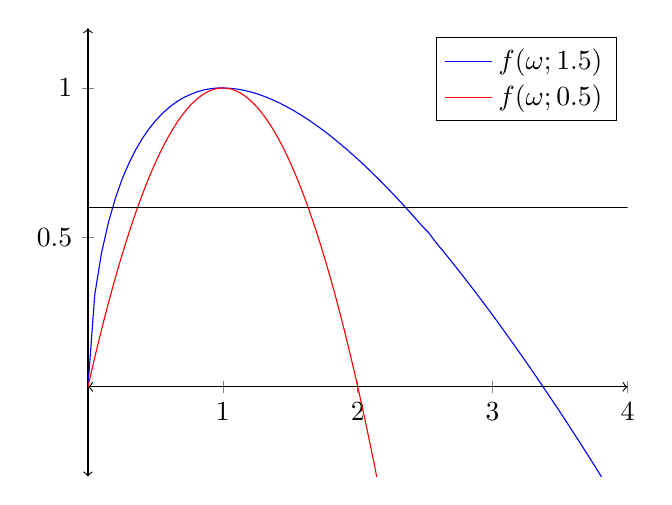
\begin{tikzpicture}
  \begin{axis}[
    xmin=0,xmax=4,
    ymin=-0.3,ymax=1.2,
    axis lines=center,
    axis line style=<->]
    \def\elas{1.5}
    \def\elass{0.5}
    \addplot[-] expression[domain=0:5,samples=100,color=blue]{(\elas*x/abs(x)*abs(x)^(1/\elas)-x))/(\elas-1)}; 
    \addplot[-] expression[domain=0:3,samples=100,color=red]{(\elass*x/abs(x)*abs(x)^(1/\elass)-x))/(\elass-1)}; 
    \addplot[mark=none, black, samples=2] {0.6};
    \legend{$f(\omega;\elas)$,$f(\omega;\elass)$};
  \end{axis}
\end{tikzpicture}

To solve for $f(\omega;\varepsilon) - (1-b) = 0$, can use Newton's method
\[\omega' = \omega - \frac{\varepsilon\omega^\frac{1}{\varepsilon} - \omega + (1-\varepsilon)(1-b)}{\omega^{\frac{1}{\varepsilon}-1}-1} = \frac{(1-\varepsilon)(\omega^{\frac{1}{\varepsilon}}-1+b)}{\omega^{\frac{1}{\varepsilon}-1}-1}\]

Choice between two different expenditures:

\[U(E) > U(E') \Leftrightarrow \frac{\theta (E/p)^{1-\frac{1}{\varepsilon}}}{1-\frac{1}{\varepsilon}} - E + b(E)> \frac{\theta (E'/p)^{1-\frac{1}{\varepsilon}}}{1-\frac{1}{\varepsilon}} - E' + b(E')\]

or

\[\frac{\theta p^{1-\frac{1}{\varepsilon}}}{1-\frac{1}{\varepsilon}} \left(E^{1-\frac{1}{\varepsilon}} - {E'}^{1-\frac{1}{\varepsilon}}\right) > E-E' -b(E) + b(E')\]

or 

\[\frac{\varepsilon\omega^{\frac{1}{\varepsilon}}}{\varepsilon-1} \left(1 - \left(\frac{E'}{E}\right)^{1-\frac{1}{\varepsilon}}\right) > 1-\frac{E'}{E} - b + b'\frac{E'}{E}\]

When consumers choose a ``non-optimal" quantity of choice $j$, the likelihood is
\begin{align*}
l &= Pr\left(U_j(E) > U^*_j \land U_j(E) > \max(U_k(E), U_k^*)\right) \\
&= Pr(U_j(E) > U^*_j) \times Pr\left(U_j(E) > \max(U_k(E), U_k^*)\mid U_j(E) > U^*_j\right)
\end{align*}

The condition $U_j(E) > U^*_j$ is equivalent to $\omega \in [\omega_l, \omega_h]$. Thus, the probability $Pr\left(U_j(E) > \max(U_k(E), U_k^*)\mid U_j(E) > U^*_j\right)$ can be estimated with simulation by drawing from the truncated distribution of $\omega$.

When consumers choose the optimal quantity instead:
\begin{align*}
l &= Pr\left(E_j^* \land U^* > U_j(E) \land U^* > \max(U_k(E), U_k^*)\right) \\
&= Pr(E_j^* \land U^* > U_j(E)) \times  Pr\left(U_j(E) > \max(U_k(E), U_k^*) \mid E_j^* \land U^* > U_j(E) \right)
\end{align*}

Draw $r$: $(p_{jr}, \theta_{jr})$

\end{document}